\lhead[\thepage]{CAPÍTULO \thechapter. PATRONES DE PARALELISMO}
\chead[]{}
\rhead[Patrones de programación paralelos de alto nivel en arquitecturas de memoria distribuida\leftmark]{\thepage}
\renewcommand{\headrulewidth}{0.5pt}

\lfoot[]{}
\cfoot[]{}
\rfoot[]{}
\renewcommand{\footrulewidth}{0pt}

%% This is an example first chapter.  You should put chapter/appendix that you
%% write into a separate file, and add a line \include{yourfilename} to
%% main.tex, where `yourfilename.tex' is the name of the chapter/appendix file.
%% You can process specific files by typing their names in at the 
%% \files=
%% prompt when you run the file main.tex through LaTeX.
\chapter{Patrones de paralelismo}
\label{ch:patrones_paralelismo}
\markboth{}{PATRONES DE PARALELISMO}

Este capítulo presenta los patrones de paralelismo, qué son y cuales son sus principales casos de uso. Primero, explicamos que son los patrones de paralelismo (Sección \ref{sec:patrones_paralelismo_introduccion}). Después, presentamos los principales patrones y su formalización matemática (Sección \ref{sec:descripcion_patrones}). Finalmente, se describen los patrones implementados en \acrshort{grppi} y las posibilidades de composición entre patrones que ofrece \acrshort{grppi} (Sección \ref{sec:interfaz_patrones_grppi}). 

\section{Introducción}
\label{sec:patrones_paralelismo_introduccion}

Los patrones pueden definirse vagamente como estrategias comúnmente recurrentes para tratar problemas particulares. Esta metodología ha sido ampliamente utilizada en múltiples áreas, como arquitectura, programación orientada a objetos y arquitectura de software. En nuestro caso, aprovechamos los patrones para el diseño de software paralelo, ya que ha sido reconocido como una de las mejores prácticas de codificación. Esto se debe principalmente a que los patrones proporcionan un mecanismo para encapsular características algorítmicas, haciéndolas más robustas, portátiles y reutilizables, mientras que si se adaptan, pueden lograr una mejor escalabilidad y ubicación de datos. En general, los patrones paralelos se pueden categorizar en dos grupos: patrones paralelos de streaming, por ejemplo, Pipeline, Farm y Filter; y datos paralelos, por ejemplo, Map, Reduce y MapReduce. Siguiendo esta clasificación, describimos formalmente los patrones soportados por nuestra interfaz en la siguiente Sección.


\section{Descripción de los patrones y formalización matemática}
\label{sec:descripcion_patrones}

En esta Sección describimos formalmente los patrones paralelos de streaming (\emph{Pipeline, Farm, Filter y Accumulator}) y los patrones de datos paralelos (\emph{Map, Reduce, Stencil, MapReduce y Divide\&Conquer}), todos ellos incluídos en \acrshort{grppi}.

\subsection{Patrones de streaming}

\begin{itemize}
    \item \textbf{Pipeline}: Este patrón procesa los elementos que aparecen en el flujo de entrada en varias etapas paralelas. Cada etapa de este patrón procesa los datos producidos por la etapa anterior en la tubería y entrega los resultados a la siguiente. Siempre que la etapa $i$-ésima en un pipe con  $n$-etapas compute la función $f_i:\alpha \to \beta$, el Pipeline entrega el elemento $x_i$ a la secuencia de salida aplicando la función $f_n(f_{n-1}(\ldots f_1(x_i) \ldots ))$. El principal requisito de este patrón es que las funciones relacionadas con las etapas deben ser puras, es decir, pueden computarse en paralelo sin efectos secundarios.
    

\vspace{0.35cm}    
    \begin{figure}[htb]
    \centering
    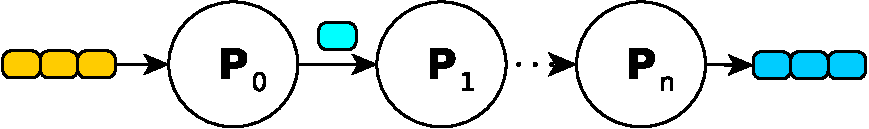
\includegraphics[width=0.40\textwidth]{figures/pipeline.pdf}
    \caption{Patrón Pipeline.}
    \label{fig:chap3:Pipeline}
    \end{figure}
\vspace{0.35cm}
    
    \item \textbf{Farm}: Este patrón computa en paralelo la siguiente función: $f: \alpha \rightarrow \beta$ sobre todos los items que aparecen en la secuencia de entrada. Por lo tanto, para cada elemento $x_i$ en la secuencia de entrada, el patrón Farm entrega el elemento a la secuencia de salida como $f(x_i)$. En este patrón, los cálculos realizados por $f$ para los elementos en el flujo de entrada deben ser completamente independientes entre sí, de lo contrario no pueden procesarse en paralelo. 
    
    \vspace{0.35cm}
    \begin{figure}[htb]
    \centering
    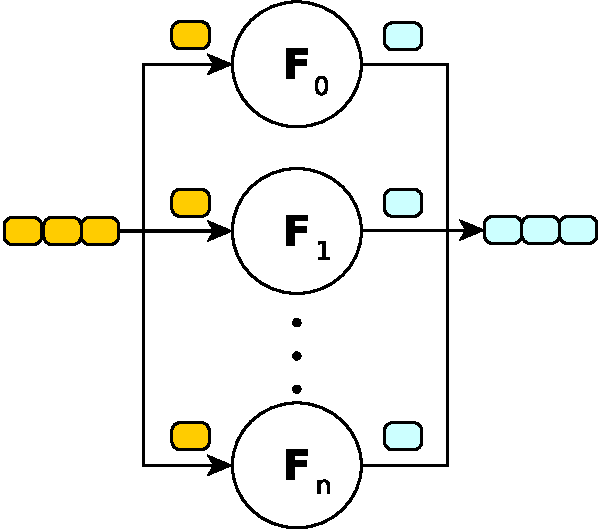
\includegraphics[width=0.30\textwidth]{figures/farm.pdf}
    \caption{Patrón Farm.}
    \label{fig:chap3:Farm}
    \end{figure}
    \vspace{0.35cm}
    
    \item \textbf{Filter}: Este patrón calcula en paralelo un filtro sobre los elementos que aparecen en la secuencia de entrada, pasando solo a la secuencia de salida aquellos elementos que satisfacen la función booleana ``filter'' (o predicado) $\mathcal{P}:\alpha \rightarrow \{true, false\}$. Básicamente, el patrón recibe una secuencia de elementos de entrada $\ldots, x_{i+1}, x_i,$ $x_{i-1}, \ldots$ y produce una secuencia de elementos de salida del mismo tipo pero con diferente cardinalidad. La evaluación de la función de filtrado en un elemento de entrada debe ser independiente de cualquier otra, es decir, el predicado debe ser una función pura. 
    
    \vspace{0.35cm}
    \begin{figure}[htb]
    \centering
    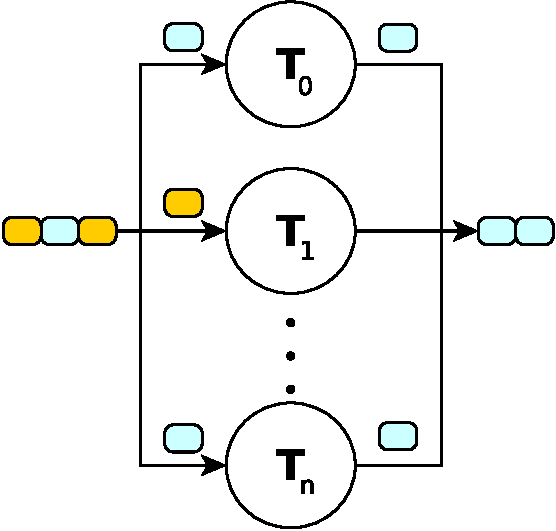
\includegraphics[width=0.30\textwidth]{figures/filter.pdf}
    \caption{Patrón Filter.}
    \label{fig:chap3:filter}
    \end{figure}
    \vspace{0.35cm}
    
    \item \textbf{Accumulator}: Este patrón colapsa los elementos que aparecen en la secuencia de entrada y entrega estos resultados a la secuencia de salida. La función utilizada para contraer los valores de elemento $\oplus$ debe ser una función binaria pura de tipo $\oplus:\alpha \times \alpha \to \alpha$, siendo generalmente asociativa y conmutativa. Básicamente, el patrón calcula la función $\oplus$ sobre una secuencia finita de elementos de entrada $\ldots, x_{i+1}, x_i, x_{i-1}, \ldots$ para producir un elemento contraído en la secuencia de salida . La cantidad de elementos que se acumulará depende del tamaño de ventana configurado como parámetro.
    
    \vspace{0.35cm}
    \begin{figure}[htb]
    \centering
    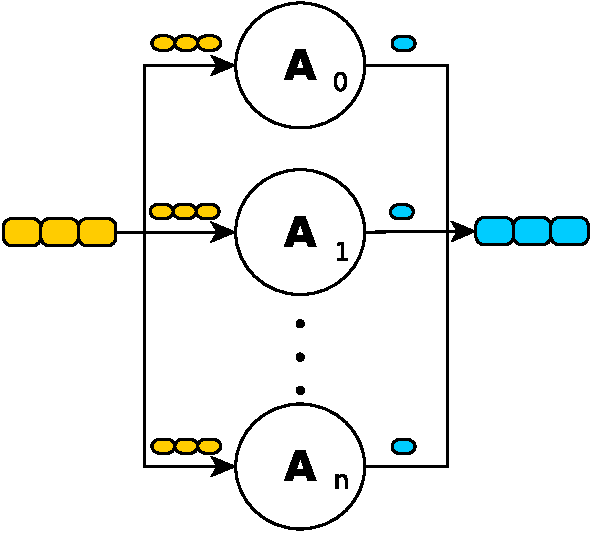
\includegraphics[width=0.30\textwidth]{figures/accumulator.pdf}
    \caption{Patrón Accumulator.}
    \label{fig:chap3:accumulator}
    \end{figure}
    \vspace{0.35cm}
    
\end{itemize}

\subsection{Patrones de datos}

\begin{itemize}
   \item \textbf{Map}: Este patrón paralelo de datos calcula la función $f: \alpha \rightarrow \beta$ sobre los elementos de la colección de datos de entrada, donde los elementos de entrada y salida son de los tipos $\alpha$ y $\beta$ respectivamente. El resultado de salida es la colección de elementos $y_{1}, y_{2}, \ldots, y_{N}$, donde $y_{i} = f(x_{i})$ para cada $i = 1, 2, \ldots, N$ y $x_{i}$ el el elemento $i$-ésimo de la colección de entrada. El único requisito del patrón map es que la función $f$ sea pura. 
   
   \vspace{0.35cm}
   \begin{figure}[htb]
    \centering
    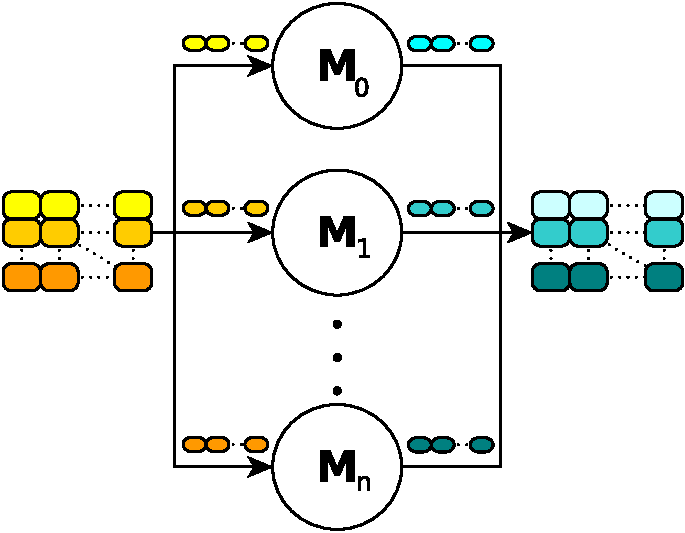
\includegraphics[width=0.35\textwidth]{figures/map.pdf}
    \caption{Patrón Map.}
    \label{fig:chap3:map}
    \end{figure}
    \vspace{0.35cm}
    
    \item \textbf{Reduce}: Este patrón paralelo de datos agrega los elementos de la colección de datos de entrada de tipo $\alpha$ utilizando la función binaria $\oplus: \alpha \times \alpha \to \alpha $, que generalmente es asociativa y conmutativa. Finalmente, el resultado del patrón se resume en un solo elemento $y$ del tipo $\alpha$ que se obtiene al realizar la operación $y = x_{1} \oplus x_{2} \oplus \ldots x_{N}$, donde $x_{i}$ es el elemento $i$-ésimo de la colección de datos de entrada. La principal restricción de este patrón es que la función binaria debe ser pura.
    
    \vspace{0.35cm}
    \begin{figure}[htb]
    \centering
    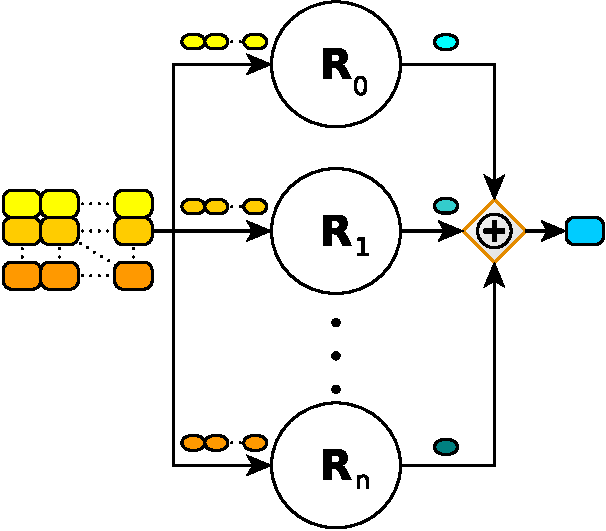
\includegraphics[width=0.3\textwidth]{figures/reduce.pdf}
    \caption{Patrón Reduce.}
    \label{fig:chap3:reduce}
    \end{figure}
    \vspace{0.35cm}

    \item \textbf{Stencil}: Este patrón es una generalización del patrón map en el cual una función elemental puede acceder, no solo a un elemento único en una colección de entrada, sino también a un conjunto de vecinos. La función $f: \alpha* \rightarrow \alpha$ utilizada por el patrón stencil recibe el elemento de entrada y un conjunto de vecinos ($\alpha*$) y produce un elemento de salida del mismo tipo. El principal requisito de este patrón es que la función $f$ debe ser pura. 
    
    \vspace{0.35cm}
    \begin{figure}[htb]
    \centering
    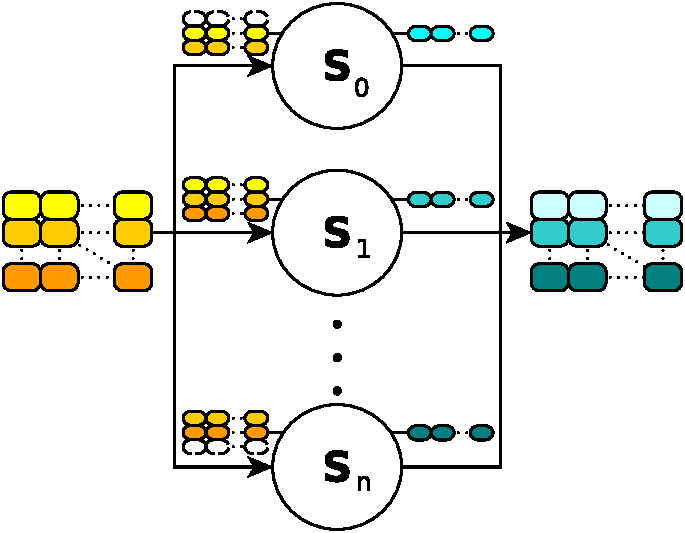
\includegraphics[width=0.35\textwidth]{figures/stencil.pdf}
    \caption{Patrón Stencil.}
    \label{fig:chap3:stencil}
    \end{figure}
    \vspace{0.35cm}
    
    \item \textbf{MapReduce}: Este patrón calcula, en una primera etapa, un patrón tipo map, una función de valor de clave sobre todos los elementos de una colección de entrada, y entrega, en una segunda etapa, un patrón de reducción, un conjunto de pares de valores de clave únicos donde el valor asociado a la clave es la ``suma'' de los valores emitidos para la misma clave. Para hacerlo, el patrón mapreduce calcula en la función map $f : \alpha \rightarrow \{\alpha, Key\}$ los elementos en la colección de entrada; luego usa la función binaria de reducción $\oplus: \beta \times \beta \to \beta$ para resumir los resultados parciales con la misma clave. El resultado de este patrón es una colección de elementos de datos de tipo $\beta$, uno por clave. Los requisitos del patrón mapreduce es que las funciones relacionadas tanto map como reduction deben ser puras.
    
    \vspace{0.35cm}
    \begin{figure}[htb]
    \centering
    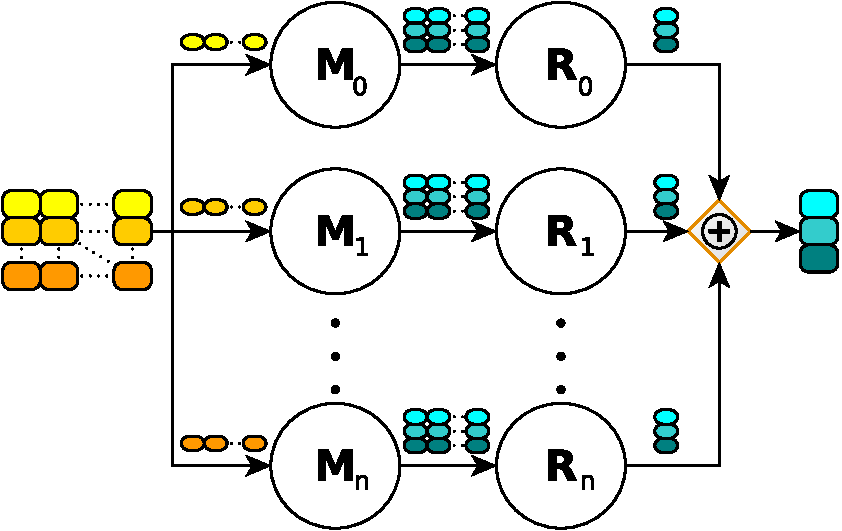
\includegraphics[width=0.40\textwidth]{figures/mapreduce.pdf}
    \caption{Patrón MapReduce.}
    \label{fig:chap3:mapreduce}
    \end{figure}
    \vspace{0.35cm}
    
    \item \textbf{Divide\&Conquer}: Este patrón calcula un problema dividiéndolo en dos o más subproblemas del mismo tipo hasta que se alcanza el caso base y se resuelve directamente. Después, las soluciones de los subproblemas se combinan para proporcionar una solución al problema original. En otras palabras, este patrón aplica la función $f : \alpha * \rightarrow \beta * $ en una colección de elementos de tipo $\alpha$ y produce una colección de elementos de tipo $\beta$. Una función de división $\mathcal{D}$ se usa primero para dividir la colección en distintas particiones hasta el tamaño del problema base, que se puede resolver directamente aplicando $f$. Finalmente, los resultados parciales de los problemas de base se combinan de acuerdo con una función de combinación $\mathcal{M}$ para construir la colección de salida final. Los requisitos del patrón dac es que las funciones $f$, $\mathcal{S}$ y $\mathcal{M}$ deben ser puras. 
    
    \vspace{0.35cm}
    \begin{figure}[htb]
    \centering
    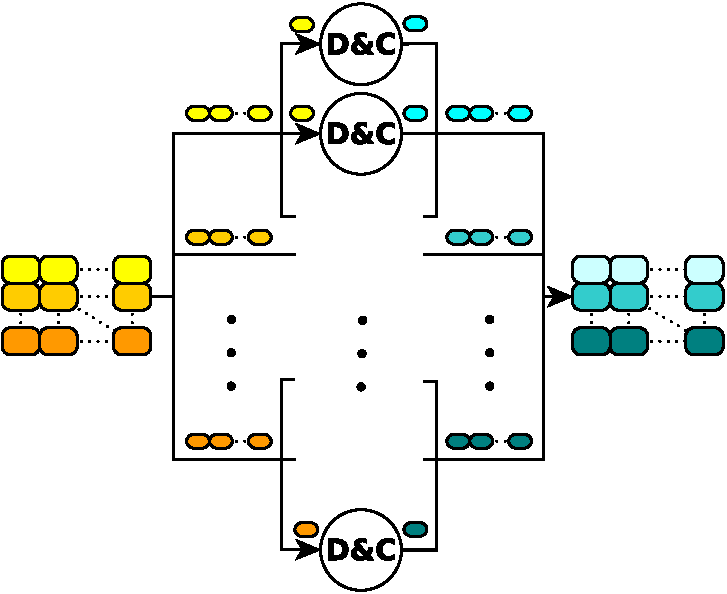
\includegraphics[width=0.40\textwidth]{figures/divideandconquer.pdf}
    \caption{Patrón Divide\&Conquer.}
    \label{fig:chap3:divideandconquer}
    \end{figure}
    \vspace{0.35cm}
    
\end{itemize}

\section{Interfaz de los patrones en \acrshort{grppi}}
\label{sec:interfaz_patrones_grppi}

En esta sección se presenta la interfaz de patrones paralelos genérica y reutilizable (\acrshort{grppi}) para aplicaciones C ++. \acrshort{grppi} aprovecha al máximo las características modernas de C ++, los conceptos de metaprogramación y la programación genérica para actuar como un interruptor entre los modelos de programación paralelos \acrshort{openmp}, hilos C ++, Intel \acrshort{tbb} y \acrshort{cuda} Thrust. Su diseño permite a los usuarios aprovechar los frameworks de ejecución antes mencionados solo en una interfaz única y compacta, ocultando la complejidad detrás del uso de mecanismos de concurrencia. Además, la modularidad de \acrshort{grppi} permite integrar fácilmente nuevos patrones, combinándolos para organizar otros más complejos. Gracias a esta propiedad, \acrshort{grppi} se puede utilizar para implementar una amplia gama de aplicaciones existentes de procesamiento de datos y de flujo de datos con esfuerzos relativamente pequeños, teniendo como resultado códigos portátiles que se pueden ejecutar en múltiples frameworks. La Figura \ref{fig:chap3:grppi} representa la vista general de la biblioteca \acrshort{grppi}.

\vspace{0.35cm}
\begin{figure}[htb]
    \centering
    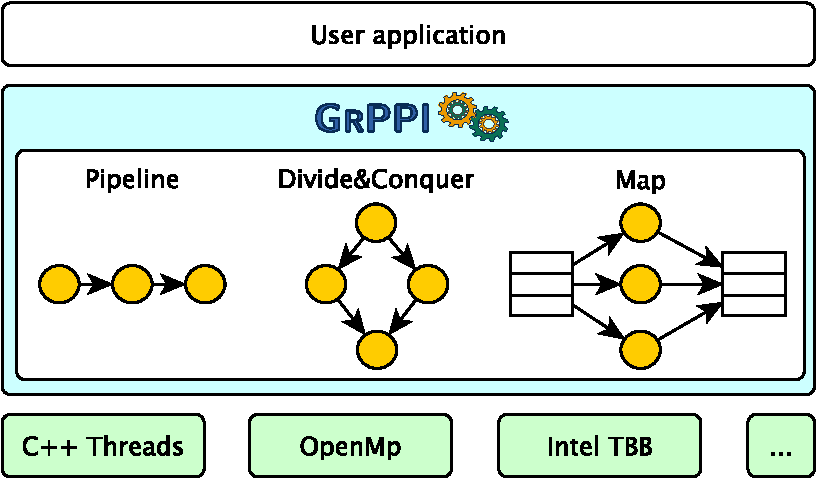
\includegraphics[width=0.60\textwidth]{figures/grppi.pdf}
    \caption{Arquitectura de \acrshort{grppi}.}
    \label{fig:chap3:grppi}
    \end{figure}
    \vspace{0.35cm}

A continuación, describimos en detalle las interfaces de los patrones paralelos ofrecidos por \acrshort{grppi} y demostrar su capacidad de compilación a través de diferentes ejemplos simples.

\subsection{Descripción de las interfaces}

\acrshort{grppi} ofrece patrones de streaming y patrones de datos con una única interfaz cuidadosamente diseñada para permitir la composición y admitir múltiples back-ends de implementación.

\subsubsection{Patrones de streaming}

Los patrones de streaming incluídos en \acrshort{grppi} son Pipeline, Farm, Filter y Accumulator.

\begin{itemize}
    \item \textbf{Pipeline}: La interfaz \acrshort{grppi} diseñada para el patrón Pipeline recibe el modelo de ejecución y las funciones (\texttt{in} y \texttt{stages}) relacionadas con sus etapas. Como se puede ver en el Listado \ref{code:Pipeline}, su interfaz C ++ usa plantillas, haciéndola más flexible y reutilizable para cualquier tipo de datos. Tenga en cuenta también el uso de plantillas variadicas, lo que permite que una tubería tenga un número arbitrario de etapas al recibir una colección de objetos invocables pasados como argumentos. En \acrshort{grppi}, la implementación paralela de este patrón se lleva a cabo utilizando un conjunto de entidades concurrentes, cada una de las cuales se ocupa de una sola etapa. Esto se controla a través del parámetro del modelo de ejecución, que se puede configurar para operar en secuencia o en paralelo, a través de los diferentes frameworks compatibles; p.ej. para usar \acrshort{openmp}, el parámetro debe establecerse en \texttt{parallel\_execution\_omp}.
    
    \vspace{0.35cm}
    \begin{lstlisting}[frame=single,label={code:Pipeline},caption={Interfaz Pipeline.}]
template <typename ExecMod, typename InFunc, typename ... Arguments>
void Pipeline( ExecMod m, InFunc const &in, Arguments ... stages );
\end{lstlisting}
\vspace{0.35cm}

    \item \textbf{Farm}: De forma similar, la interfaz del patrón Farm, que se muestra en el Listado \ref{code:Farm}, recibe el modelo de ejecución y tres funciones (\texttt{in}, \texttt{Farm} and \texttt{out}) que son a cargo de \emph{i)} consumir los artículos del flujo de entrada, \emph{ii)} procesarlos individualmente, y \emph{iii)} entregar los resultados al flujo de salida. Tenga en cuenta que la función \texttt{Farm} se ejecutará en paralelo por las diferentes entidades concurrentes. En este caso, el modelo de ejecución puede recibir opcionalmente, como argumento, el número de entidades que se utilizarán para la ejecución paralela, por ejemplo, \texttt{parallel\_execution\_omp\{6\}} utiliza 6 hilos de trabajo \acrshort{openmp}. Si no se proporciona este argumento, la interfaz toma por defecto el número de hilos establecidos por la plataforma subyacente.
    
    \vspace{0.35cm}
    \begin{lstlisting}[frame=single,label={code:Farm},caption={Interfaz Farm.}]
template <typename ExecMod, typename InFunc, typename TaskFunc, typename OutFunc>
void Farm( ExecMod m, InFunc const &in, TaskFunc const &Farm, OutFunc const &out );
\end{lstlisting}
\vspace{0.35cm}
    
    \item \textbf{Filter}: La interfaz para el patrón filter, que se describe en el Listado \ref{code:filter}, recibe el argumento del modelo de ejecución, seguido de un consumidor de flujo (\texttt{in}), filtro (\texttt{filter}) y productor (\texttt{out}). Específicamente, la función \texttt{in} lee elementos de la secuencia de entrada y los reenvía a la función \texttt{filter} que es responsable de determinar si un elemento debe ser aceptado o no. Posteriormente, los elementos que satisfacen la rutina de filtrado son recibidos por la función \texttt{out} para entregarlos al flujo de salida. Tenga en cuenta que es obligatorio que la función \texttt{filter} devuelva una expresión booleana. La implementación paralela de este patrón aplica la función de filtro usando un conjunto de entidades concurrentes, que se pueden configurar en el parámetro del modelo de ejecución.
    
    \vspace{0.35cm}
    \begin{lstlisting}[frame=single,label={code:filter},caption={Interfaz Filter.}]
template <typename ExecMod, typename InFunc, typename FilterFunc, typename OutFunc>
void Filter( ExecMod m, InFunc const &in, FilterFunc const &filter, OutFunc const &out );
\end{lstlisting}
\vspace{0.35cm}
    
    \item \textbf{Accumulator}: El patrón accumulator tiene como objetivo reducir, utilizando una función de reducción específica (\texttt{redop}) los elementos que aparecen en el flujo de entrada. De forma similar a las otras interfaces, la interfaz del acumulador, como se muestra en el Listado \ref{code:accum}, recibe el modelo de ejecución; la función de consumidor de flujo (\texttt{in}) el tamaño de la ventana, es decir, el número de elementos que formarán parte de cada operación de reducción; el desplazamiento, que determina el número de elementos superpuestos entre las ventanas; el operador de reducción; y una función de productor (\texttt{out}) responsable de entregar los artículos al flujo de salida. En este caso, las entidades concurrentes en la implementación paralela son responsables de procesar individualmente la acumulación de las ventanas de flujo de entrada.
    
    \vspace{0.35cm}
    \begin{lstlisting}[frame=single,label={code:accum},caption={Interfaz Accumulator.}]
template <typename GenFunc, typename ReduceOperator, typename OutFunc>
void Accumulator( ExecMod m, GenFunc const &in, int windowsize, int offset, ReduceOperator const &redop, OutFunc const &out );
\end{lstlisting}
\vspace{0.35cm}
    
\end{itemize}

\subsubsection{Patrones de datos}

Los patrones de datos incluídos en \acrshort{grppi} son Map, Reduce, Stencil, MapReduce y Divide\&Conquer.

\begin{itemize}
    \item \textbf{Map}: La interfaz \acrshort{grppi} para el patrón map, que se muestra en el Listado~\ref{code:map}, ecibe los siguientes parámetros de entrada: el modelo de ejecución, las referencias al primer y último elemento de las colecciones de datos de entrada y la función kernel (\texttt{map}). Después del cálculo, el resultado del patrón del mapa se deja en la posición correspondiente del conjunto de datos de salida. Dado que cada elemento de la colección de datos de entrada es independiente entre sí, la ejecución paralela del patrón de mapa se puede realizar de la siguiente manera. Primero, la colección de entrada se divide por igual entre las entidades concurrentes disponibles. Posteriormente, estas entidades ejecutan en paralelo la función kernel \texttt{map} y escriben los resultados en los segmentos correspondientes de la recopilación de datos de salida.
    
    \vspace{0.35cm}
    \begin{lstlisting}[frame=single,label={code:map},caption={Interfaz Map.}]
template <typename ExecMod, typename InputIt, typename OutputIt, typename TaskFunc, typename ... MoreIn>
void Map(ExecMod m, InputIt first, InputIt last, OutputIt firstOut, TaskFunc const &map, MoreIn ... inputs );
\end{lstlisting}
\vspace{0.35cm}
    
    \item \textbf{Reduce}: La interfaz para el patrón reduce, como se describe en el Listado~\ref{code:reduce}, toma el modelo de ejecución, una referencia al primer y último elemento de la colección de datos de entrada y al operador de reducción. El resultado de la reducción se escribe en el parámetro de salida pasado por referencia. De acuerdo con las propiedades del operador de reducción, el cálculo de reducción se puede realizar en paralelo. Por lo tanto, la recopilación de datos de entrada se divide en $N$ trozos y se calcula en paralelo mediante $N$ entidades concurrentes diferentes que producen un conjunto de resultados parciales. Finalmente, el resultado del patrón de reducción se calcula en serie por una de estas entidades.
    
    \vspace{0.35cm}
    \begin{lstlisting}[frame=single,label={code:reduce},caption={Interfaz Reduce.}]
template <typename ExecMod, typename InputIt, typename Output, typename ReduceOperator>
void Reduce(ExecMod m, InputIt first, InputIt last, Output &out, ReduceOperator const &redop);
\end{lstlisting}
\vspace{0.35cm}
    
    \item \textbf{Stencil}: La interfaz \acrshort{grppi} para el patrón stencil, presentado en el Listado~\ref{code:stencil}, es bastante similar a la del patrón de mapa, con la excepción de que también recibe la función de vecindad  (\texttt{nh}). Esta función es responsable de acceder a los vecinos en una determinada coordenada del conjunto de datos de entrada. La implementación paralela del patrón de esténcil es análoga a la del patrón de mapa. Sin embargo, el acceso a los vecinos en los límites de un conjunto de datos particionados podría requerir comparaciones adicionales entre las posiciones de los elementos.
    
    \vspace{0.35cm}
    \begin{lstlisting}[frame=single,label={code:stencil},caption={Interfaz Stencil.}]
template <typename ExecMod, typename InputIt, typename OutputIt, typename TaskFunc, typename NFunc, typename ... MoreIn>
void Stencil(ExecMod m, InputIt first, InputIt first, InputIt last, OutputIt firstOut, TaskFunc const &stencil, NFunc const &nh, MoreIn ... inputs);
\end{lstlisting}
\vspace{0.35cm}
    
    \item \textbf{MapReduce}: La interfaz para el patrón mapreduce combina llamadas internas al mapa y reduce las interfaces del patrón \acrshort{grppi}. En cuanto a los parámetros de entrada, recibe el modelo de ejecución, referencias al primer y último elemento de las colecciones de datos de entrada, la función kernel  (\texttt{map}) y el operador de reducción para el patrón reduce. El resultado finalmente se deja en una referencia al primer elemento de la colección de salida. La implementación paralela de este patrón en \acrshort{grppi} explota el paralelismo ofrecido internamente por el mapa y reduce los patrones paralelos. El resultado de la operación del mapa se baraja y se reduce en paralelo, uno para todos los elementos con la misma clave. El resultado global para cada clave finalmente se reduce en serie por una de las entidades concurrentes.
    
    \vspace{0.35cm}
    \begin{lstlisting}[frame=single,label={code:mapreduce},caption={Interfaz MapReduce.}]
template <typename ExecMod, typename InputIt, typename Output, typename MapFunc, typename ReduceOperator, typename ... MoreIn>
void MapReduce(ExecMod m, InputIt first, InputIt last, Output &out, MapFunc const &map, ReduceOperator const &redop, MoreIn ... inputs);
\end{lstlisting}
\vspace{0.35cm}
    
    \item \textbf{Divide\&Conquer}: La interfaz diseñada para el patrón Divide\&Conquer consta de los siguientes elementos: el modelo de ejecución, una referencia de la colección de datos de entrada y las funciones \texttt{divide}, \texttt{base\_case} and \texttt{merge}. El resultado de este patrón se escribe en la recopilación de datos de salida pasada por referencia. La implementación paralela de este patrón en la interfaz \acrshort{grppi} aprovecha primero el núcleo dividido para dividir el problema de manera constante en otros más pequeños. Esta operación es realizada por las entidades concurrentes disponibles hasta que se alcanza la dimensión de problema mínima y donde se aplica el kernel de solución de caso base. Tomando las soluciones parciales generadas, las entidades concurrentes fusionan los resultados en una estructura basada en árbol hasta que se obtiene la solución global. Tenga en cuenta que dado que el ancho del árbol puede crecer por encima del número máximo de entidades concurrentes especificadas, se usa un grupo de tareas para implementar un enfoque de programación dinámica.
    
    \vspace{0.35cm}
    \begin{lstlisting}[frame=single,label={code:dac},caption={Interfaz Divide\&Conquer.}]
template <typename ExecMod, typename Input, typename Output, typename DivFunc, typename TaskFunc, typename MergeFunc>
void DivideAndConquer(ExecMod m, Input &problem, Output &out, DivFunc const &divide, TaskFunc const &base_case, MergeFunc const &merge);
\end{lstlisting}
\vspace{0.35cm}
    
\end{itemize}

\subsection{Composición de patrones}

Como se mencionó previamente, los patrones ofrecidos por \acrshort{grppi} pueden componerse entre ellos para producir estructuras más complejas y para unir construcciones específicas presentes en aplicaciones secuenciales y paralelas de datos. Para demostrar esta característica, describimos tres ejemplos de compibilidad de patrones abordando cada una de las combinaciones factibles de paradigmas computacionales (streaming y datos) soportados por la interfaz \acrshort{grppi}: stream-stream, data-data y composición stream-data.

Para la composición del patrón stream-stream, el código en el Listado\ref{code:stream-stream-comp} implementa un Pipeline en el que la segunda etapa es un patrón Farm. Las etapas del Pipeline, pasadas como funciones lambda, realizan las siguientes tareas: \emph{i)} leer las líneas de un archivo de entrada con valores separados por espacios en blanco y empaquetarlos en una estructura vectorial, \emph{ii)} calcular el valor máximo de vectores entrantes usando el patrón Farm, y \emph{iii)} imprime los valores máximos de los vectores en un flujo de salida. Dado que el Pipeline recibe el modelo de ejecución paralela \acrshort{openmp} (línea 1), las etapas se calculan en paralelo por los 3 hilos de trabajo. De forma similar, el patrón de conjunto anidado se ejecuta mediante 6 hilos \acrshort{openmp}. Tenga en cuenta también que las variables \texttt {std::optional}, de \emph{c++ Library Fundamentals Extensions} (ISO / IEC 19568: 2015), se utilizan para marcar el final de las secuencias con un valor vacío. Denotamos esta composición de Pipeline-Farm \texttt{(\,p\,$|$\,f\,$|$\,p\,)}, siendo \texttt{p} y \texttt{f}, respectivamente, etapas secuenciales y basadas en Farm. Como se puede ver, gracias al uso de técnicas de metaprogramación, plantillas y expresiones lambda, es posible componer fácilmente patrones paralelos \acrshort{grppi} para construir otros más complejos.

\vspace{0.35cm}
\begin{lstlisting}[frame=single,label={code:stream-stream-comp},caption={Ejemplo de composición Pipeline-Farm.}]
Pipeline( parallel_execution_omp,
    // Stage 0: read values from a file
    [&]() -> optional<vector<int>> {
        auto r = read_list(is);
        return ( r.size() == 0 ) ? {} : r; 
    },
    // Stage 1: takes the maximum value of the vector
    Farm(parallel_execution_omp{6}, 
        []( vector<int> v ) {
            return ( v.size() > 0 ) ? 
                max_element(v.begin(), v.end()) : 
                numeric_limits<int>::min();
    }),
    //Stage 2: prints out the result
    [&os]( int x ) {
        os << x << endl;
    }
);
\end{lstlisting}
\vspace{0.35cm}

Con respecto a la composición del patrón de datos de datos, el Listado~\ref{code:data-data-comp} muestra una construcción donde se compone un patrón map con una operación reduce. En este caso, la matriz de entrada en el patrón map se divide en particiones iguales entre los hilos del trabajador. A continuación, para cada fila en una partición, el patrón reduce anidado resume sus valores y almacena el resultado en la posición correspondiente del vector de salida, pasado como un argumento en la llamada a la función del map. Tenga en cuenta que el modelo de ejecución en paralelo para el patrón map es \acrshort{openmp}, mientras que el patrón reduce anidado utiliza subprocesos de C ++, cada uno de ellos utilizando 6 subprocesos de trabajo. Denotamos esta composición como \texttt{m(r)}, siendo \texttt{m} y \texttt{r} los patrones map y reduce, respectivamente.

\vspace{0.35cm}
\begin{lstlisting}[frame=single,label={code:data-data-comp},caption={Ejemplo de composición Map-Reduce.}]
Map( parallel_execution_omp{6},
    // Input matrix
    mat_in.begin(), mat_in.end(),
    // Vector of accumulated values from matrix rows
    vec_out.begin(),
    // Map kernel: divide matrix into rows
    [&]( auto row_in, auto sum ) {
        // Reduce kernel: Sum up the values in a matrix row
        Reduce( parallel_execution_thr{6},
            row_in.begin(), row_in.end(), 
            &sum, 
            std::plus<double> );
        );
    }
);
\end{lstlisting}
\vspace{0.35cm}

Como se mencionó, también podemos componer stream con patrones de datos. Esta es una composición factible, dado que los elementos provenientes de un flujo se pueden procesar utilizando un patrón paralelo de datos. Sin embargo, lo contrario no es factible ya que los resultados generados en un patrón de datos no pueden transformarse en flujo y, por lo tanto, procesarse utilizando un enfoque de procesamiento de streaming. Para ilustrar una composición de patrón de datos de flujo, el Listado~\ref{code:stream-data-comp} muestra un ejemplo donde un patrón paralelo de flujo de granja se compone con un dato de Divide\&Conquer. En este caso particular, el patrón de Farm lee constantemente los valores almacenados en un archivo y calcula, para cada uno de ellos, su correspondiente \emph{i}-ésimo número de Fibonacci utilizando el patrón Divide\&Conquer. Finalmente, los números de Fibonacci se imprimen para el usuario final. Como se muestra, la paralelización de la granja se realiza utilizando 6 hilos \acrshort{openmp}, mientras que el patrón Divide\&Conquer anidado usa 6 hilos C ++. Dado que cada uno de los subprocesos relacionados con la granja crean 6 anidados en C ++, el número total de subprocesos que computan esta composición es 36. Esta composición se denota como \texttt{f(d)}, siendo \texttt{f} y \texttt{d}, los patrones Farm y Divide\&Conquer, respectivamente.

\vspace{0.35cm}
\begin{lstlisting}[frame=single,label={code:stream-data-comp},caption={Ejemplo de composición Farm-Divide\&Conquer.}]
Farm(parallel_execution_omp(6),
    [&]() -> optional<int> {  // Read values from an input file
        auto value = read_value(is);
        return ( value > 0 ) ? value : {};
    },
    [&]( int value ) { // Compute the fibonacci number using a D&C pattern    
        int fibonacci = 0;
        DivideAndConquer(parallel_execution_thr(6), value, &fibonacci,
            [&](auto &value){
                std::vector< int > subproblem;
                if( v < 2 ) subproblem.push_back(value);
                else        subproblem.insert(subproblem.end(), { value-1, value-2 });
                return subproblem;
            },
            [&](auto &problem, auto &partial){
                partial = ( problem == 0 ) ? 0 : 1;
            },
            [&](auto & partial, auto & out){
                out += partial;
            }
        );
        return fibonacci;
    },
    [&]( int fibonacci ) {  // Print the fibonacci values 
        cout << fibonacci << endl;
    }
);
\end{lstlisting}
\vspace{0.35cm}

En general, las Tablas ~\ref{tab:stream-stream-comp}, ~\ref{tab:data-data-comp} y ~\ref{tab:stream-data-comp} resumen las composiciones de patrones agrupadas por las tres posibles combinaciones de paradigmas computacionales compatibles con la interfaz \acrshort{grppi}: stream-stream, data-data y stream-data. Tenga en cuenta que las filas y columnas en las tablas representan los patrones externos e internos involucrados en una composición determinada, respectivamente. Clasificamos cada composición de patrón específico con una de las siguientes cuatro categorías, desde menos hasta más restrictivas:

\begin{itemize}
    \item \textbf{No-Factible}: Esta categoría representa una composición que no es compatible con \acrshort{grppi}.
    \item \textbf{Factible}: Esta categoría denota una composición que se puede implementar en \acrshort{grppi}.
    \item \textbf{Irreducible}: esta categoría es una composición factible que proporciona un patrón paralelo útil que no puede simplificarse más. Tenga en cuenta que las composiciones de patrones que se incluyen en esta categoría son compatibles de forma nativa con \acrshort{grppi}.
    \item \textbf{Usable-Reducible}: Esta categoría es una composición factible que implementa una composición de patrones que puede simplificarse aún más, pero que, en algunos casos, proporciona un código más claro y más legible que su equivalente más simple.
\end{itemize}

Como se muestra en la Tabla~\ref{tab:stream-stream-comp}, las composiciones de patrones stream-stream que involucran un Pipeline y otro patrón se clasifican como Irreducible (excepto aquellos con un patrón de accumulator externo), dado que no es posible obtener la misma construcción paralela usando un patrón más simple. Este tipo de composiciones son compatibles nativamente en \acrshort{grppi}, como se muestra en el Listado~\ref{code:stream-stream-comp}. Cualquier otra composición se considera Factible ya que pueden simplificarse usando el patrón externo o interno con un mayor grado de paralelismo. Sin embargo, estas construcciones no proporcionan ninguna ventaja importante en comparación con la construcción más simple. Por otro lado, las composiciones que contienen un patrón de acumulador externo son No-Factible, ya que este patrón no recibe ninguna función de usuario para ejecutarse en paralelo.

\vspace{0.35cm}
\begin{table}[htbp]
\centering
%\resizebox{\textwidth}{%
\caption{Composiciones stream-stream.}
\begin{adjustbox}{max width=\textwidth}
\begin{tabular}{@{}ccccc@{}}
\toprule
 & Pipeline & Farm & Filter & Accumulator \\ 
\midrule
Pipeline  & \feasim     & \irredm     & \irredm     & \irredm     \\
\midrule
Farm      & \irredm     & \feasim     & \feasim     & \feasim     \\
\midrule
Filter    & \irredm     & \feasim     & \feasim     & \feasim     \\
\midrule
Accumulator     & \nfeasm     & \nfeasm     & \nfeasm     & \nfeasm     \\
\bottomrule
\end{tabular}
\end{adjustbox}
\label{tab:stream-stream-comp}
\end{table}
\vspace{0.35cm}


Centrándose en las composiciones de datos de datos, como se muestra en la Tabla~\ref{tab:data-data-comp}, las construcciones cuyo patrón exterior es similar a un map (map and stencil) se categorizan como Usable-Reducible. Esto se debe a que existe un equivalente más simple que usa solo el patrón externo tipo mapa. En cuanto al patrón de reducción, no se puede combinar con ningún otro interno. Las razones son las mismas que para el patrón del acumulador en las composiciones de flujo continuo. Otras composiciones cuyo patrón exterior es mapreduce o Divide\&Conquer se clasifican como Factible, ya que pueden implementarse en \acrshort{grppi} aunque no aportan ninguna ventaja importante.

\vspace{0.35cm}
\begin{table}[htbp]
\centering
%\resizebox{\textwidth}{%
\caption{Composiciones data-data.}
\begin{adjustbox}{max width=\textwidth}
\begin{tabular}{@{}cccccc@{}}
\toprule
 & Map       & Reduce    & Stencil   & MapReduce & Divide\&Conquer      \\
\midrule
Map       & \usablm     & \usablm     & \usablm     & \usablm     & \usablm     \\
\midrule
Reduce    & \nfeasm     & \nfeasm     & \nfeasm     & \nfeasm     & \nfeasm     \\
\midrule
Stencil   & \usablm     & \usablm     & \usablm     & \usablm     & \usablm     \\
\midrule
MapReduce & \feasim     & \feasim     & \feasim     & \feasim     & \feasim     \\
\midrule
Divide\&Conquer & \feasim     & \feasim     & \feasim     & \feasim     & \feasim     \\
\bottomrule
\end{tabular}
\end{adjustbox}
\label{tab:data-data-comp}
\end{table}
\vspace{0.35cm}

Finalmente, las composiciones de stream-data se resumen en la Tabla~\ref{tab:stream-data-comp}. Las composiciones cuyo patrón exterior es Pipeline o Farm se denotan como Irreducible. La combinación de dos paradigmas paralelos distintos (stream-data) hace que estas composiciones sean únicas e impide que se simplifiquen más. En cuanto a las composiciones con un patrón de filtro externo, la cardinalidad de salida de su patrón interno determina si la composición es Factible or Usable-Reducible. Esto se debe a que la salida de la función de filtro es booleana. 

\vspace{0.35cm}
\begin{table}[htbp]
\centering
%\resizebox{\textwidth}{%
\caption{Composiciones stream-data.}
%\resizebox{\textwidth}{!}{
\begin{adjustbox}{max width=\textwidth}
\begin{tabular}{@{}cccccc@{}}
\toprule
 & Map       & Reduce    & Stencil   & MapReduce & Divide\&Conquer      \\
\midrule
Pipeline  & \irredm     & \irredm     & \irredm     & \irredm     & \irredm     \\
\midrule
Farm      & \irredm     & \irredm     & \irredm     & \irredm     & \irredm     \\
\midrule
Filter    & \feasim     & \feasim*    & \feasim     & \feasim     & \feasim*    \\
\midrule
Accumulator & \nfeasm     & \nfeasm     & \nfeasm     & \nfeasm     & \nfeasm     \\
\bottomrule
\end{tabular}
\end{adjustbox}
%}
\label{tab:stream-data-comp}
\end{table}
\vspace{0.35cm}

Por ejemplo, en una composición map-filter, la cardinalidad de salida del patrón map es igual a la cardinalidad de entrada. De modo que, aunque el predicado del patrón filter se puede implementar transformando el conjunto de datos de salida en un booleano, este caso no refleja una práctica común. Por lo tanto, clasificamos estas composiciones solo como Factible. Por otro lado, la cardinalidad de salida del patrón reduce en una composición filter-reduce es un elemento único. Por lo tanto, el predicado de filtro se puede implementar fácilmente transformando dicho elemento en un booleano. Por esta razón, categorizamos esta construcción como un caso especial de composición Factible. La combinación filter-Divide\&Conquer también es un caso especial de composición Factible porque la cardinalidad de salida del patrón Divide\&Conquer depende del algoritmo. Finalmente, el patrón accumulator no se puede componer y, por lo tanto, es clasificado como No-Factible.





%\afterpage{\blankpage} % blank page
